%!TEX TS-program = xelatex  
%!TEX encoding = UTF-8 Unicode  
      
\documentclass[a4paper,10pt]{article}
\usepackage[top=1.0in, bottom=1.0in, left=1.0in, right=1.0in]{geometry} 
\usepackage{indentfirst}        
\usepackage{float}
\usepackage{amsmath}
\usepackage{hyperref}
\usepackage{graphicx}

\title{ARMA-GARCH}
\author{SHIHENG SHEN}
\date{\today}
\begin{document}
\maketitle

\section{Temperature Model}
\subsection{Objective}
Build a robust time series model to forecast future temperature's interval. 


\subsection{Data Source}
HadCRUT4 is a gridded dataset of global historical surface temperature anomalies relative to a 1961-1990 reference period. Data are available for each month since January 1850, on a 5 degree grid. \url{http://www.metoffice.gov.uk/hadobs/hadcrut4/data/current/time_series/HadCRUT.4.5.0.0.monthly_ns_avg.txt}.

\subsection{Data adjustment}
From the shown url, grab the monthly global mean of temperature anomalies from 1850-2016, which amounts to a length of 2004. Using decompose() function in R to get the adjusted value.(See appendix)  

\subsection{Road Map}
We went through a lot of difficulties during the construction of a proper model. Below is the basic idea I've thinked about.\par
\begin{itemize}
\item Dealing with Statonarity: diff() or time trend(linear, dynamic linear, discrete fourier series)?
\item Dealing with stochastic volatility: taking logarithm or exclude some data or both? Stochastic volatility model?
\item Choosing model: ARIMA or ARFIMA or ARMA-sGARCH or ARMA-eGARCH or ARFIMA-sGARCH or ARFIMA-eGARCH?
\end{itemize}

\subsection{Starting from \textit{arima} model}
First, examine the stationarity of $myTS.adjusted$. Strange enough, it passed the $adf.test$ despite that it has a clear trend, as shown in the figure. So we tried to use $auto.arima()$ to decide if it is $I(1)$ or $I(0)$. As shown in the code and results, a $arima(2, 1, 4)$ model fits $myTS.adjusted$ better in both $acf$ and $pacf$. The t-value of the coefficients of $auto.arima(residuals)$ is smaller for $arima(2, 1, 4)$.\par
The forecast of $arima(2, 1, 4)$ for 240 months from $2017.1$ is shown in the figure. Within the sample, we compare the forecast and the actual data, only to find that $arima(2, 1, 4)$ is far from satisfying. 

\subsection{Long-Memory Model}
Though acf shows that some lags are significant, but we think it's only because we took too big a confidential level. Actually the problem is not that great, but we still build a $ARFIMA$ model. \par
We plot the $acf$ of the residuals of $ARFIMA$ model, but it seems that $ARFIMA$ can't effectively explain our data.

\subsection{Solving Heterodasticity: Standard GARCH}
Looking at the plot of the residuals of $arima(2, 1, 4)$. Obviously there exists heterodasticity problem. Using $adf.test$, it supports our doubt. Therefore we have the motive to build a $GARCH$ model. We decide to use the package $rugarch$.\par
A standard GARCH model has the following variance equation:
\begin{equation*}
	\sigma_t^2 = (w + \sum_{j = 1}^m \zeta_j v_{jt}) + \sum_{j = 1}^q \alpha_j \varepsilon_{t-j}^2 + \sum_{j = 1}^p \beta_j \sigma_{t-j}^2
\end{equation*} 
\indent We wrote a function to test different order for the model as shown in appendix. Due to the problem that rugarch package only deals with stationary series, we first $diff()$ $myTS.adjusted$. After trying a few times from $(1, 0), (0, 0, 0)$ to $(5, 5), (4, 0, 4)$, \textit{GARCH(1 ,1), ARIMA(2, 0, 3)} is the most satisfying model. Here we realize that using GARCH model, the order of ARIMA might changes. 
\indent Substract the standardized(w.r.t. the variance model) residuals $z$, which is $z = \cfrac{residuals(fit)}{sigma(fit)}$. Plot $z$, we'll find $z$ seems to have a far smoother variance. Just for fun, plot a normal sample series with the same parameters. We'll find in the two figures it's hard to distinguish between the two. Looking at the $LM-Test$ in the summary of $fit 1$, the heterodasticity is wiped out at lower lags.  More graphical diagnostics is available in the figure appendix. From these diagnostics we find sGARCH is to some extent a proper model.
\indent Since we difference the series at first, now forecast becomes more complex. We have to calculate the variance by adding all the terms' variance.




\newpage
\section{Appendix}

\subsection{R Code}
\subsubsection{Data Adjustment}
\begin{verbatim}
library(curl)
tmpf <- tempfile()
curl_download(url, tmpf)
gtemp <- read.table(tmpf)[, 1:2]
temp = gtemp$V2[1:2004]
library(TSA)
myTS = ts(as.numeric(temp), start = c(1850, 1), frequency = 12)
myTS.additive = decompose(myTS)
myTS.adjusted = as.numeric(myTS.additive$x - myTS.additive$seasonal)
\end{verbatim}



\subsubsection{arima models}
\begin{verbatim}
> tseries::adf.test(myTS.adjusted)

	Augmented Dickey-Fuller Test

data:  myTS.adjusted
Dickey-Fuller = -5.1646, Lag order = 12, p-value = 0.01
alternative hypothesis: stationary

> library(forecast)
> auto.arima(myTS.adjusted)
Series: myTS.adjusted 
ARIMA(2,1,4)(2,0,1)[12] with drift         

Coefficients:
         ar1     ar2      ma1      ma2     ma3     ma4    sar1    sar2     sma1
      0.5041  0.3585  -1.0458  -0.1600  0.1362  0.0779  0.7619  0.0779  -0.7884
s.e.  0.2432  0.2143   0.2424   0.3482  0.1082  0.0257  0.0926  0.0248   0.0910
      drift
      5e-04
s.e.  2e-04

sigma^2 estimated as 0.01428:  log likelihood=1417.03
AIC=-2812.05   AICc=-2811.92   BIC=-2750.43

> arima1 = Arima(myTS.adjusted, c(2, 0, 1))
> auto.arima(arima1$residuals)
Series: arima1$residuals 
ARIMA(5,1,0)(2,0,1)[12]                    

Coefficients:
          ar1      ar2      ar3      ar4      ar5    sar1    sar2     sma1
      -0.8556  -0.6256  -0.4849  -0.3136  -0.1475  0.7647  0.0837  -0.7907
s.e.   0.0224   0.0287   0.0299   0.0286   0.0222  0.0846  0.0248   0.0831

sigma^2 estimated as 0.01705:  log likelihood=1238.65
AIC=-2459.29   AICc=-2459.2   BIC=-2408.87

> arima2 = Arima(myTS.adjusted, c(2, 1, 4))
> auto.arima(arima2$residuals)
Series: arima2$residuals 
ARIMA(1,0,1)(2,0,1)[12] with non-zero mean 

Coefficients:
         ar1      ma1    sar1    sar2     sma1    mean
      0.5645  -0.5685  0.7389  0.0745  -0.7672  0.0062
s.e.  2.5541   2.5131  0.1253  0.0244   0.1242  0.0033

sigma^2 estimated as 0.01427:  log likelihood=1417.4
AIC=-2820.81   AICc=-2820.75   BIC=-2781.59

# looking at acf
# Choose arima(2, 1, 4)
> tseries::adf.test(arima2$residuals)

	Augmented Dickey-Fuller Test

data:  arima2$residuals
Dickey-Fuller = -11.777, Lag order = 12,
p-value = 0.01
alternative hypothesis: stationary

> arima2
Series: myTS.adjusted 
ARIMA(2,1,4)                    

Coefficients:
         ar1     ar2      ma1      ma2     ma3     ma4
      0.5129  0.3271  -1.0438  -0.1331  0.1166  0.0748
s.e.  0.2753  0.2357   0.2748   0.3833  0.1117  0.0265

sigma^2 estimated as 0.01443:  log likelihood=1405.3
AIC=-2796.6   AICc=-2796.55   BIC=-2757.38

#forecast for future
> plot(forecast.Arima(arima2, h = 240))

# forecast within the sample and comparision
> sarima = Arima(myTS.adjusted[1:1800], c(2, 1, 4))
> plot(forecast.Arima(sarima, h = 203))
> lines(myTS.adjusted)
\end{verbatim}



\subsubsection{ARFIMA Model}
\begin{verbatim}
> lmodel = arfima(myTS.adjusted)
> summary(lmodel)

Call:
  arfima(y = myTS.adjusted) 

*** Warning during (fdcov) fit: unable to compute correlation matrix; maybe change 'h'

Coefficients:
       Estimate
d         0.445
ar.ar1    0.249
ar.ar2    0.612
ma.ma1    0.223
ma.ma2    0.549
sigma[eps] = 0.1200103 
[d.tol = 0.0001221, M = 100, h = 1.481e-05]
Log likelihood:  1404 ==> AIC = -2796.513 [6 deg.freedom]

> acf(lmodel$residuals)




\end{verbatim}

\subsubsection{sGARCH Model}
\begin{verbatim}
> arch.test(arma2$residuals)
ARCH heteroscedasticity test for residuals 
alternative: heteroscedastic 

Portmanteau-Q test: 
     order    PQ p.value
[1,]     4  99.4       0
[2,]     8 116.9       0
[3,]    12 411.5       0
[4,]    16 475.6       0
[5,]    20 495.9       0
[6,]    24 755.8       0
Lagrange-Multiplier test: 
     order   LM p.value
[1,]     4 1418       0
[2,]     8  697       0
[3,]    12  418       0
[4,]    16  212       0
[5,]    20  168       0
[6,]    24  137       0

library(rugarch)
my_sGARCH_test <- function(p, q, m, n, ts.data = res)
{
	# I use include.mean = FALSE after trying TRUE
	# to find out insignificance
    myspec=ugarchspec(variance.model = list(model = "sGARCH", garchOrder = c(p, q)), 
    	mean.model = list(armaOrder = c(m, n), include.mean = FALSE), 
    	distribution.model = "normal")
    myfit=ugarchfit(myspec,data=ts.data, solver="solnp")
    return(myfit)  
}

> dtemp = diff(myTS.adjusted)
> fit1 = my_sGARCH_test(1, 1, 2, 3, dtemp)

> fit1

*---------------------------------*
*          GARCH Model Fit        *
*---------------------------------*

Conditional Variance Dynamics 	
-----------------------------------
GARCH Model	: sGARCH(1,1)
Mean Model	: ARFIMA(2,0,3)
Distribution	: norm 

Optimal Parameters
------------------------------------
        Estimate  Std. Error    t value Pr(>|t|)
ar1    -0.090935    0.015226    -5.9724 0.000000
ar2     0.754333    0.015069    50.0583 0.000000
ma1    -0.391906    0.007313   -53.5917 0.000000
ma2    -0.863257    0.000130 -6647.5909 0.000000
ma3     0.295634    0.007800    37.9010 0.000000
omega   0.000082    0.000034     2.3956 0.016595
alpha1  0.023026    0.003614     6.3706 0.000000
beta1   0.970594    0.004705   206.2925 0.000000

Robust Standard Errors:
        Estimate  Std. Error    t value Pr(>|t|)
ar1    -0.090935    0.017031    -5.3393 0.000000
ar2     0.754333    0.017312    43.5726 0.000000
ma1    -0.391906    0.002647  -148.0378 0.000000
ma2    -0.863257    0.000144 -6000.9074 0.000000
ma3     0.295634    0.002903   101.8443 0.000000
omega   0.000082    0.000036     2.2838 0.022382
alpha1  0.023026    0.003636     6.3329 0.000000
beta1   0.970594    0.003734   259.9413 0.000000

LogLikelihood : 1512.336 

Information Criteria
------------------------------------
                    
Akaike       -1.5021
Bayes        -1.4797
Shibata      -1.5021
Hannan-Quinn -1.4939

Weighted Ljung-Box Test on Standardized Residuals
------------------------------------
                         statistic p-value
Lag[1]                      0.3742  0.5407
Lag[2*(p+q)+(p+q)-1][14]    4.5219  1.0000
Lag[4*(p+q)+(p+q)-1][24]   13.5547  0.3236
d.o.f=5
H0 : No serial correlation

Weighted Ljung-Box Test on Standardized Squared Residuals
------------------------------------
                        statistic   p-value
Lag[1]                      31.06 2.506e-08
Lag[2*(p+q)+(p+q)-1][5]     37.84 1.904e-10
Lag[4*(p+q)+(p+q)-1][9]     51.28 4.433e-13
d.o.f=2

Weighted ARCH LM Tests
------------------------------------
            Statistic Shape Scale   P-Value
ARCH Lag[3]  0.004507 0.500 2.000 9.465e-01
ARCH Lag[5] 11.085543 1.440 1.667 3.565e-03
ARCH Lag[7] 20.592184 2.315 1.543 4.509e-05

Nyblom stability test
------------------------------------
Joint Statistic:  2.6294
Individual Statistics:              
ar1    0.25019
ar2    0.61592
ma1    0.19513
ma2    0.24162
ma3    0.07259
omega  0.10095
alpha1 0.42035
beta1  0.20019

Asymptotic Critical Values (10% 5% 1%)
Joint Statistic:     	 1.89 2.11 2.59
Individual Statistic:	 0.35 0.47 0.75

Sign Bias Test
------------------------------------
                   t-value      prob sig
Sign Bias           0.3363 7.367e-01    
Negative Sign Bias  3.6815 2.380e-04 ***
Positive Sign Bias  4.4421 9.396e-06 ***
Joint Effect       33.2983 2.786e-07 ***


Adjusted Pearson Goodness-of-Fit Test:
------------------------------------
  group statistic p-value(g-1)
1    20     57.32    1.019e-05
2    30     63.59    2.167e-04
3    40     85.01    2.883e-05
4    50    102.77    1.103e-05


Elapsed time : 0.365526

> z = residuals(fit1) / sigma(fit1)
> plot.ts(z)
> mean(z)
[1] 0.03181525
> var(z)
[1] 1.013866
> length(z)
[1] 2003
> plot.ts(rnorm(2003, 0.03181525, 1.013866))

# forecast
> fore1 = ugarchforecast(fit1, n.ahead = 24)
> fore.diff = as.numeric(fore1@forecast$seriesFor)
> fore.sigma = as.numeric(fore1@forecast$sigmaFor)
> ts.predict = temp[length(temp)] + cumsum(fore.diff)
> ts.predict = ts.predict + myTS.additive$figure
> ts.sigma = sqrt(cumsum(fore.sigma^2))
> tsup.sigma = ts.predict + ts.sigma
> tsdown.sigma = ts.predict - ts.sigma
> plot(1:24, ts.predict, ylim=c(0,1.5), type = 'l', col = 'blue',
  xlab = "months", ylab = "temperature predict")
> lines(1:24, tsup.sigma, type = 'l', col = 'red')
> lines(1:24, tsdown.sigma, type = 'l', col = 'red')
\end{verbatim}




\subsection{Figures}

\begin{figure}[H]
\centering
\caption{HadCRUT4 Data Global Mean Time Series}
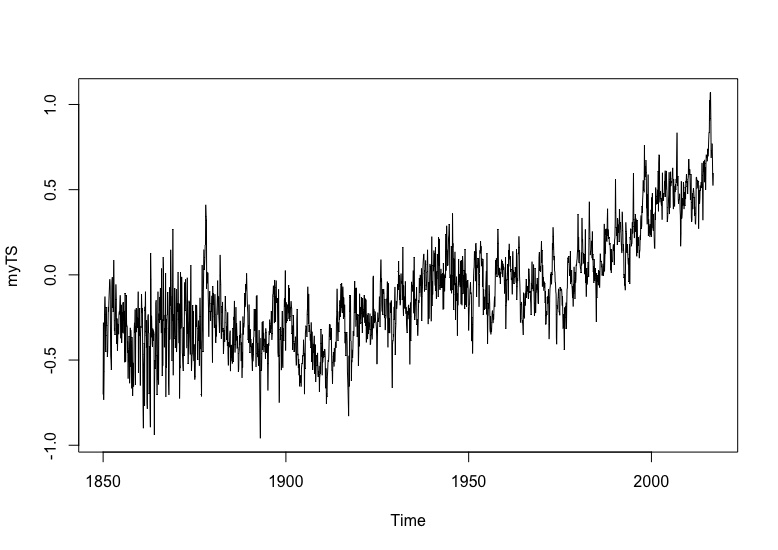
\includegraphics[scale=.5]{temp.png}
\end{figure}

\begin{figure}[H]
\centering
\caption{Plot myTS.adjusted}
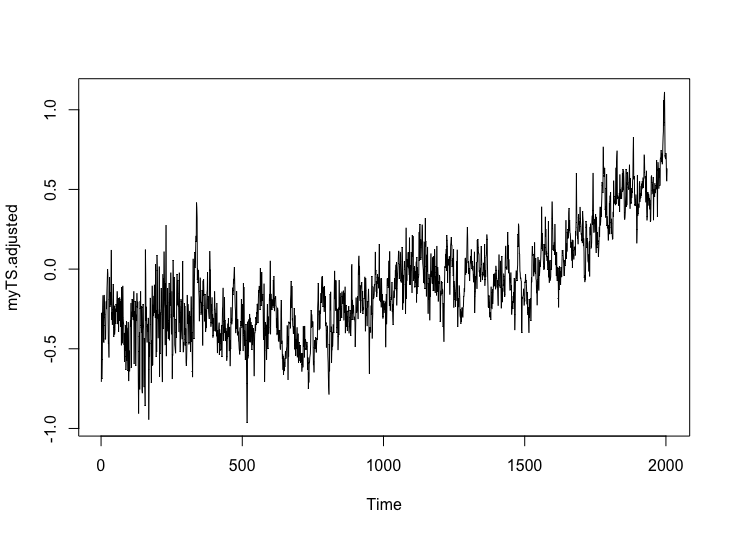
\includegraphics[scale=.5]{myTSadjusted.png}
\end{figure}

\begin{figure}[H]
\centering
\caption{Selecting arma order: acf of residuals of arma(2, 0, 1) \& (2, 1, 4)}
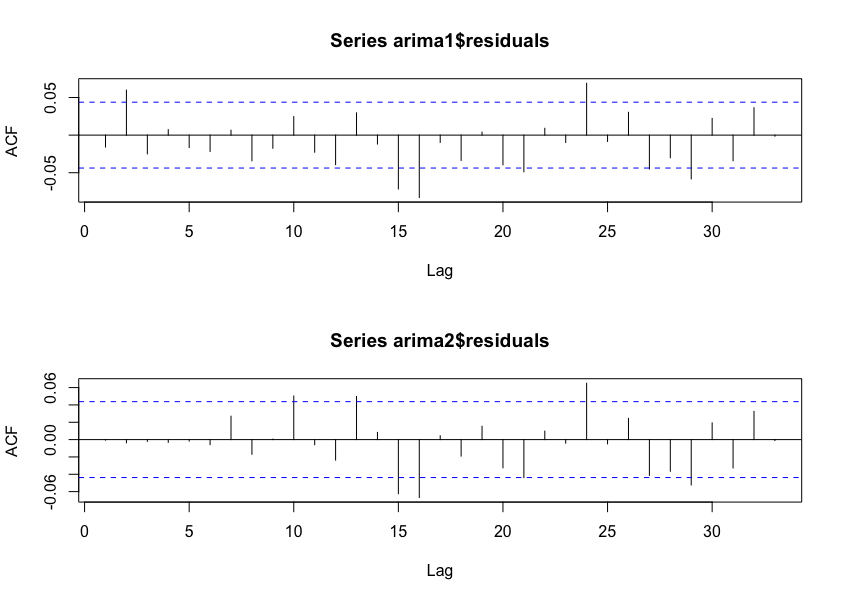
\includegraphics[scale=.5]{armaacf.png}
\end{figure}

\begin{figure}[H]
\centering
\caption{Selecting arma order: pacf of residuals of arma(2, 0, 1) \& (2, 1, 4)}
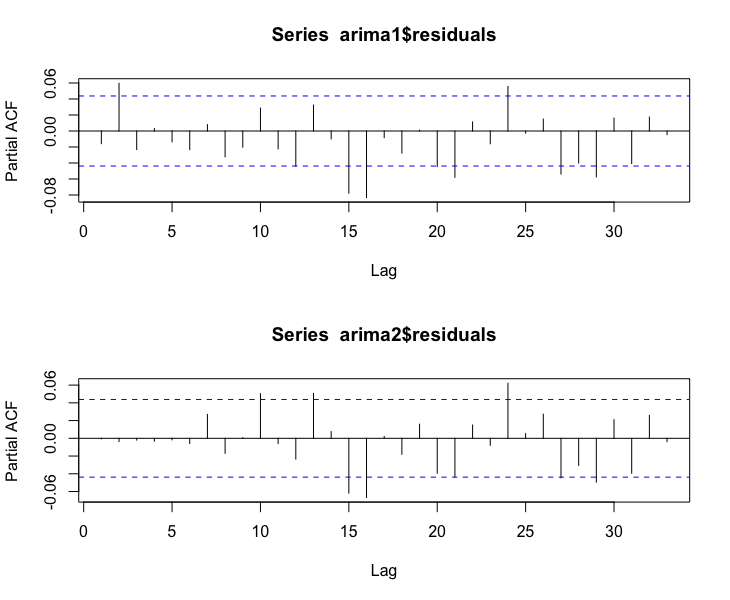
\includegraphics[scale=.5]{arima_pacf.png}
\end{figure}

\begin{figure}[H]
\centering
\caption{Forecast next 20 years(240 months) using arima(2, 1, 4)}
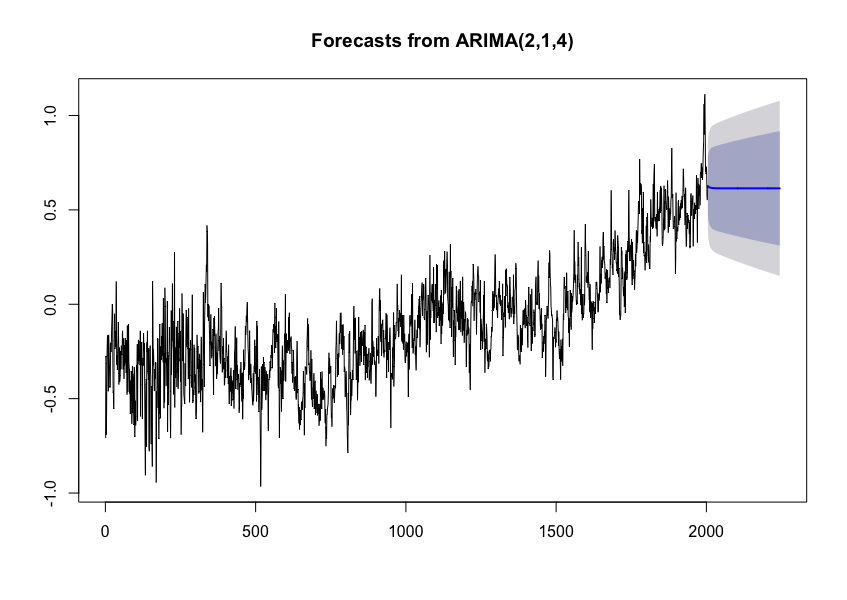
\includegraphics[scale=.5]{arima_forecast.png}
\end{figure}

\begin{figure}[H]
\centering
\caption{Forecast within the sample compared with the actual data using arima(2, 1, 4)}
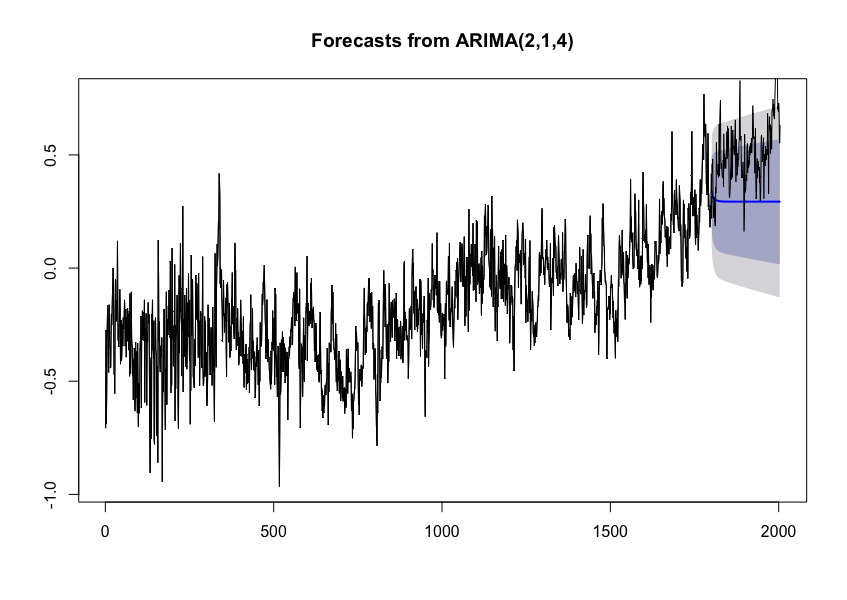
\includegraphics[scale=.5]{arima_sample.png}
\end{figure}

\begin{figure}[H]
\centering
\caption{Plot arima2's residuals}
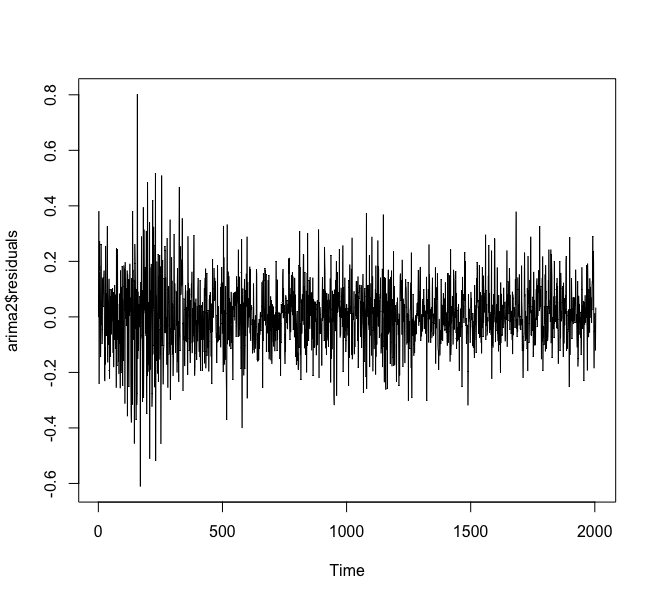
\includegraphics[scale=.5]{arima_residuals.png}
\end{figure}

\begin{figure}[H]
\centering
\caption{acf of residuals of ARFIMA}
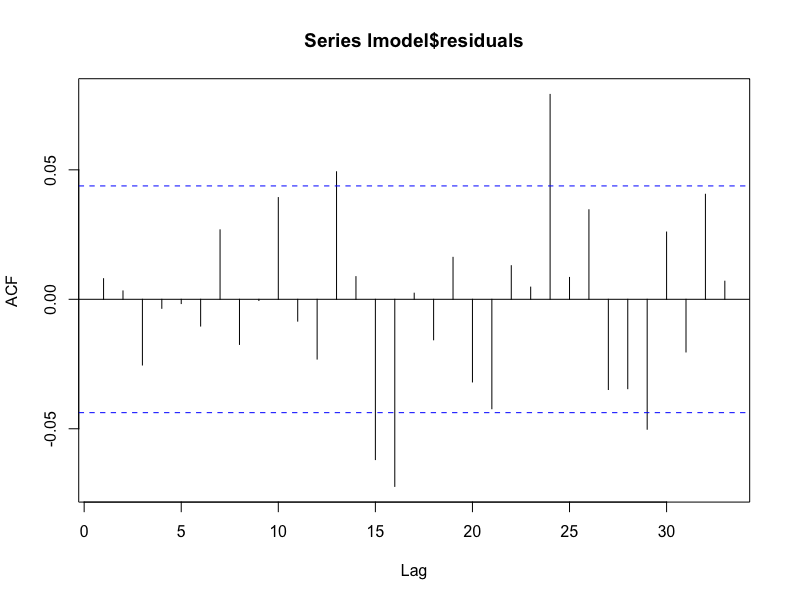
\includegraphics[scale=.5]{longacf.png}
\end{figure}


\newpage 

\begin{figure}[H]
\centering
\caption{z}
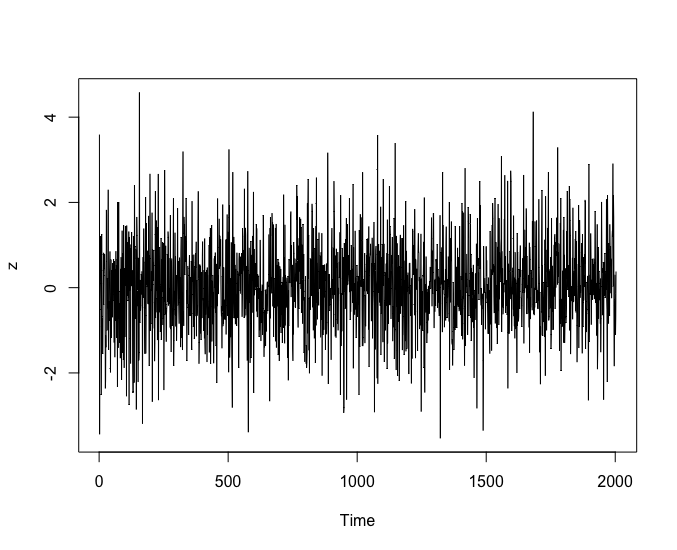
\includegraphics[scale=.40]{z.png}
\end{figure}

\begin{figure}[H]
\centering
\caption{simulation of using rnorm}
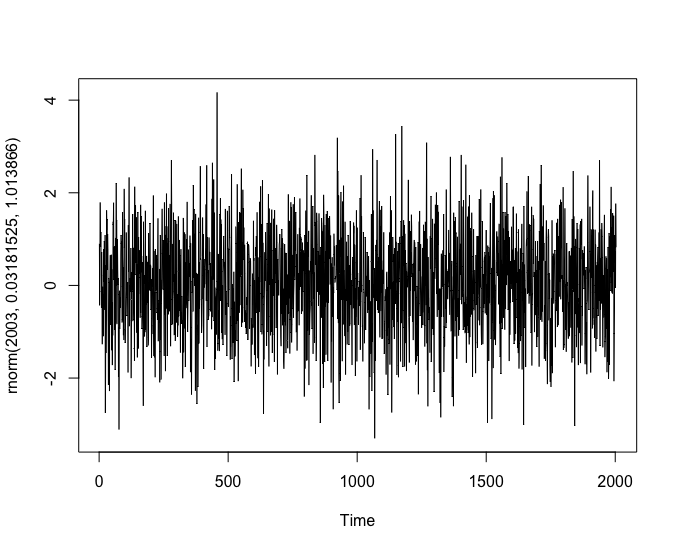
\includegraphics[scale=.40]{rnorm.png}
\end{figure}

\begin{figure}[H]
\centering
\caption{acf(z)}
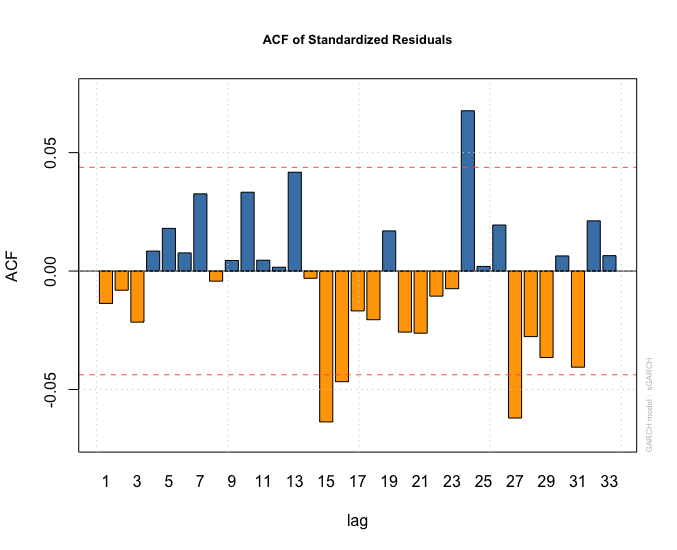
\includegraphics[scale=.50]{zacf.png}
\end{figure}

\begin{figure}[H]
\centering
\caption{Empirical Density of Standardized Residuals}
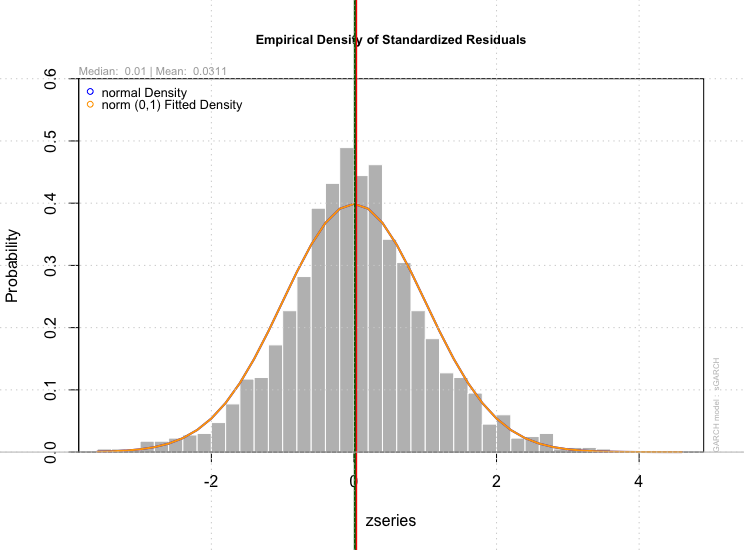
\includegraphics[scale=.60]{density.png}
\end{figure}
 

\begin{figure}[H]
\centering
\caption{qqplot of $z$}
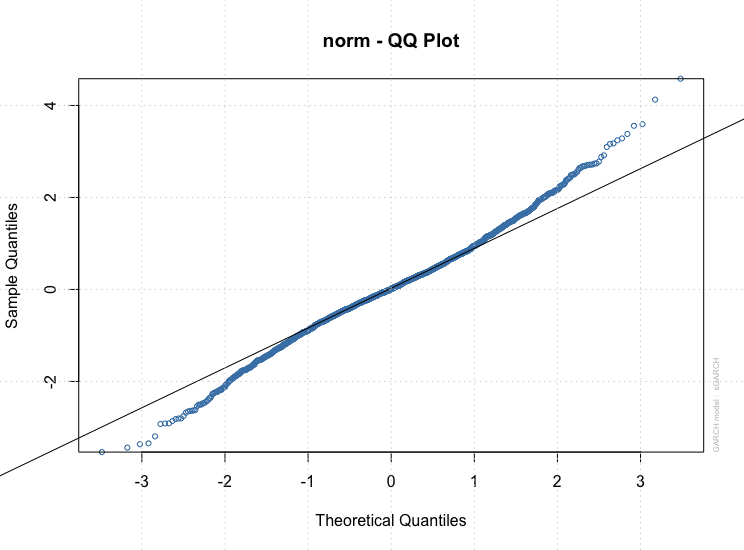
\includegraphics[scale=.60]{qqplot.png}
\end{figure}

\begin{figure}[H]
\centering
\caption{forecast for sGARCH Model}
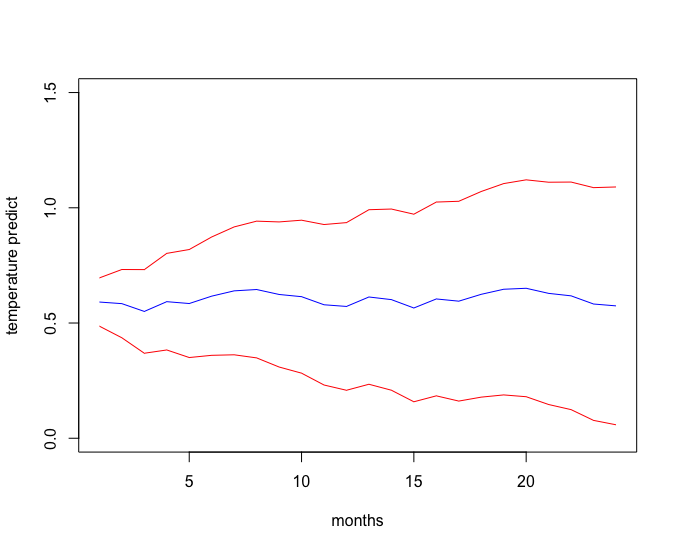
\includegraphics[scale=.60]{predict01.png}
\end{figure}

\subsection{Others}
\subsubsection{Details about \textit{decompose()} used in seasonal adjustment}
Type `decompose' in R console, we can see the source code of this function. The process of `type = additive' is listed below:
\begin{itemize}
\item the argument passed into decompose() is a `ts' object 
\item denote the argument ts(x, frequency = f). Create a filter using: filter = c(0.5, rep(1, f - 1), 0.5)/f.
\item trend = filter(x, filter)
\item season = x - trend, then compute f means of season with interval length f, the f means denoted by figure. Adjusting figure figure = figure - mean(figure)
\item seasonal is just length(x)/f times repetition of figure.
\item random = x - seasonal - trend
\end{itemize}


\end{document}